
\documentclass[a4paper]{tufte-handout}
%%%%%%%%%%%%%%
%  Packages  %
%%%%%%%%%%%%%%
\usepackage{lab_notes} 
\usepackage{pgfplots}
\usepackage{tikz}
\usepackage{hyperref}
\usepackage{minted}
\hypersetup{
    pdffitwindow=false,            % window fit to page
    pdfstartview={Fit},            % fits width of page to window
    pdftitle={Lab notes 2014},     % document title
    pdfauthor={Your Name},         % author name
    pdfsubject={},                 % document topic(s)
    pdfnewwindow=true,             % links in new window
    colorlinks=true,               % coloured links, not boxed
    linkcolor=DarkScarletRed,      % colour of internal links
    citecolor=DarkChameleon,       % colour of links to bibliography
    filecolor=DarkPlum,            % colour of file links
    urlcolor=DarkSkyBlue           % colour of external links
}


%%%%%%%%%%%%%%%
%  meta data  %
%%%%%%%%%%%%%%%
\newcommand{\userName}{Anass Belcaid}
\newcommand{\workingDate}{\today}
\title{Introduction to machine Learning. Assignment 1}
\newcommand{\institution}{Ecole Nationale Supérieure d'Arts et Métiers}
\date{\today}

\begin{document}
\maketitle

\section{Logistic Regression}%
\label{sec:logreg}

\subsection{Bayes rule}%
\label{sub:baye_s_rule}

Suppose you have a D-dimensional data vector $x=(x_1,\ldots,x_D)^T$ and an
associated class variable $y\in\{0,1\}$ which is \textbf{Bernoulli} with parameter
$\alpha$ \sidenote{ $p(y=1)=\alpha$ and $p(y=0) = 1-\alpha$}. Assume that the dimensions of $\mathbf{x}$ are conditionally
independent given $y$, and that the conditional likelihood of each $x_i$ is
Gaussian with $\mu_{i0}$ and $\mu_{i1}$ as the means of the two classes and
$\sigma_i$ as their shared standard deviation.\\
]s
Use Bayes rule to show that $p(y=1|x)$ takes the form of a logistic function:

\begin{equation}
  p(y=1|x) = \sigma(w^Tx+b) = \dfrac{1}{1 + exp\big(-\sum_{i=1}^D w_ix_i-b\big)}
\end{equation}

Derive expression for the weights $\mathbf{w}= (w_1,\ldots,w_D)^T$ and the bias
$b$ in terms of the parameters of the class likelihood and priors

Using Bayes rule we obtain\sidenote{$$ p(y|x) = \dfrac{p(x|y)p(y)}{p(x)}$$}:

\begin{equation*}
  p(y=1|x) =  \dfrac{p(x|y=1)p(y=1)}{p(x|y=1)p(y=1)+p(x|y=0)p(y=0)}
\end{equation*}

For the conditional probability $p(x|y=1)$ we use the \emph{Naive Bayes}
assumption, and we replace the probabilities for $y$:


\begin{equation}
  p(y=1|x) = \dfrac{ \prod_{i=1}^D
  p(x_i|y=1)\alpha}{\prod_{i=1}^Dp(x|y=1)\alpha+\prod_{i=1}^Dp(x|y=0)(1-\alpha)}
\end{equation}


Now we use the fact that each dimension is a Gaussian with mean $\mu_{i01}$:


\begin{equation}
  p(y=1|x) = \dfrac{ \alpha \prod_{i=1}^D
  exp\big(-\dfrac{1}{2\sigma_i^2}(x_i-\mu_{i0})^2 \big)}
  {\alpha \prod_{i=1}^D
  exp\big(-\dfrac{1}{2\sigma_i^2}(x_i-\mu_{i0})^2 \big)+
  (1-\alpha)\prod_{i=1}^D
  exp\big(-\dfrac{1}{2\sigma_i^2}(x_i-\mu_{i1})^2 \big)}
\end{equation}

Now exchanging the prod in an exponential sum and factorizing by the common
constants:

\begin{equation}
  p(y=1|x) = \dfrac{\alpha \;\exp\Big(
    \sum\big(\dfrac{x-\mu_{i0}}{\sigma_{i}}\big) \Big)}{
  \alpha \;\exp\Big(
    \sum\big(\dfrac{x-\mu_{i0}}{\sigma_{i}}\big) \Big)
  +
  (1-\alpha) \;\exp\Big(
    \sum\big(\dfrac{x-\mu_{i1}}{\sigma_{i}}\big) \Big)
  } 
\end{equation}


Now we divide by the \textbf{nominator} :

\begin{equation}
  p(y=1|x) = \dfrac{1}{1+\frac{1-\alpha}{\alpha} \exp\big(
  \dfrac{(x-\mu_{i0})^2-(x-\mu_{i1})^2}{\sigma_i}\big) }
\end{equation}


Since the \emph{standard deviation} are the same for each dimension the square
termes cancel each other and we only keep a \textbf{linear} combination of the
features in the \emph{exponential}.


\begin{equation}
  p(y=1|x) = \dfrac{1}{1+ \sum_{i=0}^D w_i x_i-b}
\end{equation}


\subsection{Maximum Likelihood estimation}%
\label{sub:maximum_likelihood}

Now suppose you are given a training set $\mathcal{D} = \left\{ (x¹,y^1),\ldots,
(x^(N),y^(N))\right\}$. Consider a binary \textbf{binary logistic regression}
classifier of same for as~\ref{sub:baye_s_rule}.\\

Derive an expression for the $E(\mathbf{w},b)$, the negative
\emph{log-likelihood} of $y$ given $x$. Then derive expressions for the
derivatives of $E$ with respect to each of the model parameters.


Let's  define the energy $E(w,b)$ and the negative log-likelihood of the
posterior probability:

\begin{equation}
  p(y=1|x) = \prod_{i=1}^N p(y=1|x^{i})
\end{equation}


We define the entities\sidenote{See Bishop(chapter 3)} $\mathbf{y}_i$
\begin{equation*}
  K_i = \sigma(Wx^{(i)} +b)
\end{equation*}

\begin{eqnarray}
  E(w,b) &=&  -\log\{p(y=1|x)\}\\
         &=& -\sum_{i=1}^N y^{(i)}\log(K_i) + (1-y^{(i)})(1-K_i) 
\end{eqnarray}
Now we derive the expression with respect to parameter $W$

\begin{equation}
  \nabla E(w,b) = \sum_{i=1}^N (y^{(i)} - K_i) x_i 
\end{equation}



\subsection{$L_2$ Regularization}%
\label{sub:_l_2_regularization}

Now assume that a Gaussian prior is placed on each element of $w$. And $b$ such
that $p(w_i) = \mathcal{N}(w_i|0, \frac{1}{\lambda})$, and $p(b)=
\mathcal{N}(b|0, \frac{1}{\lambda})$. Derive an expression that is proportional
to $p(w,b|\mathcal{D})$, the posterior distribution of $w$ and $b$ based on this
prior and the likelihood defined above. The expression you derive must contain
all terms that depend on $w$ and $b$.\\

Define $L(w,b) $ to be the negative logarithm of this posterior. Show that
$L(w,b)$ takes the following form:

\begin{equation}
  L(w,b) = E(w,b) + \frac{\lambda}{2} \sum w_i^2 +C(\lambda)
\end{equation}

where $C(\lambda)$ is a term that depends on $\lambda$ but not either on $w$ nor
$b$. What are the derivatives of $L$ with respect to each of the model
parameters.

% TODO: Deep mathematical analysis to understand the response %


\section{Logistic Regression vs KNN}%
\label{sec:logistic_regression_vs_knn}

In this section you will compare the performance and characteristics of
different classifiers, namely \textbf{Logistic Regression} and
\textbf{k-Nearest} Neighbors. You will extend the provided code and experiment
with these extensions\footnote{You should understand the code first instead of
using it as a black box}.

The data you will be working with are hand-written digits. \emph{4s} and
\emph{9s}, represented as $28\times28$ pixel arrays. There are two training
sets: 

\begin{itemize}
  \item \emph{mnist\_train} : 80 example for each class.
  \item \emph{mnist\_train\_small}: 5 example for each class
\end{itemize}

There is also a \textbf{validation} set that you should use for model selection,
and test set \emph{mnist\_test} \footnote{Code for visualizing the dataset has
been included in \emph{plot\_digits}}.\\


\subsection{subsection name}%
\label{sub:subsection_name}

Use the supplied kNN implementation to predict the labels in the
\textbf{validation} set using your normal \textbf{training} set.\\

Write a script that runs kNN for different values of $k \in\{1,3,5,7,9\}$ and
plots the classification rate\footnote{Number of correclty predicted cases,
divided by total number of data points} as a function of $k$.

\inputminted[fontsize=\tiny]{python}{../hw1_code_python/knn_cross_validation.py}
\begin{marginfigure}
  \centering
  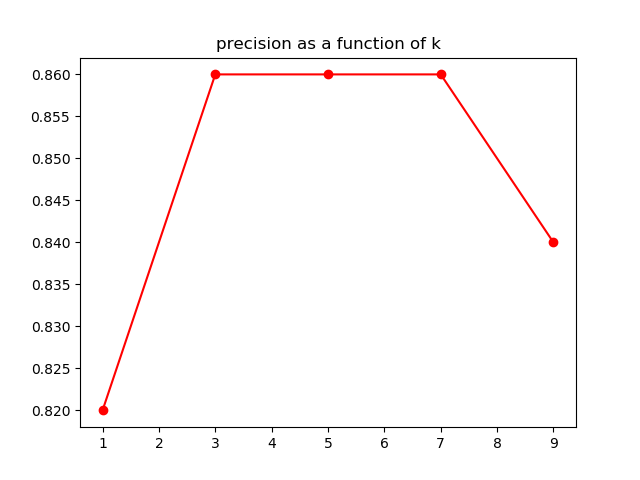
\includegraphics[width=5cm,height=5cm]{./../hw1_code_python/precisons_k.png}
  \caption{Precision as a function of K}
  \label{fig:precision}
\end{marginfigure}


\end{document}
